\documentclass[12pt,a4paper]{article}
\usepackage{amsmath}
\usepackage{graphicx}
\usepackage{circuitikz}
\usepackage{float}

\title{RC Circuit Response to Square Wave Input}
\author{Lab Experiment Report}
\date{\today}

\begin{document}

\maketitle

\section*{Objective}
To analyze the transient and steady-state responses of an RC circuit to a square wave input in three cases: \(RC = T\), \(RC >> T\), and \(RC << T\), where \(T\) is the time period of the input square wave. Input and output voltages will be observed for the first five cycles and in steady state, and theoretical values will be matched with experimental observations.

\section*{Apparatus}
\begin{itemize}
  \item Function generator
  \item Resistor 
  \item Capacitor 
  \item Oscilloscope
  \item Connecting wires
\end{itemize}

\section*{Circuit Diagram}
\begin{figure}[H]
    \centering
    \begin{circuitikz}
        \draw
        (0,0) node[ground] {}
        to[vsourcesin, l=\(\pm 5V\)] (0,3) -- (1,3)
        to[R, l=\(R\)] (3,3)
        to[short] (3,2)
        to[C, l=\(C\)] (3,0) -- (0,0) {}
        (3,2) -- (5,2)
        to[R, l=\(r\)] (5,0) -- (0,0);
    \end{circuitikz}
    \caption{RC Circuit for Square Wave Input}
    \label{fig:circuit}
\end{figure}
Image of the actual circuit we connected on the breadboard is below,
\newline
\framebox[\textwidth]{\parbox{0.95\textwidth}{Attach circuit image here.}}

\section*{Theory}

\section*{Procedure}
\begin{enumerate}
    \item Construct the circuit as shown in the above figures.
    \begin{enumerate}
        \item Connect the positive end of the function generator in series with a resistor
        \item Connect the capacitor and a small resistance in parallel, connect the combination in series with the rest of the circuit.
    \end{enumerate}
    \item Set the function generator to output a square wave with $5V$ amplitude (Peak Voltage $V$, Minimum Voltage $0V$) and a specific frequency $T$.
    Select the type of cycle as \textit{N-CYCLES}.
    \item On the second channel of function generator, tune it to output the same wave as the first channel with the exact same configurations (even burst mode, manual trigger). Connect this to the second channel of the oscilloscope. This channel will serve to compare output of voltage across capacitor with input square wave.
    \item This configuration enables the generation of a square wave with a predefined number of cycles when the trigger button is pressed on the function generator.
    On the oscilloscope, press the \textit{SINGLE} button. This ensures that the next event captured by the oscilloscope is displayed and then the display pauses automatically.
    \item Trigger the burst mode manually on the function generator to generate the single pulse or event.
    \item Observe and record the captured waveforms on the oscilloscope.
\end{enumerate}

\section*{Results}
%\pagebreak
\subsection*{Case 1: \(RC << T\)}
\begin{figure*}[h!]
    {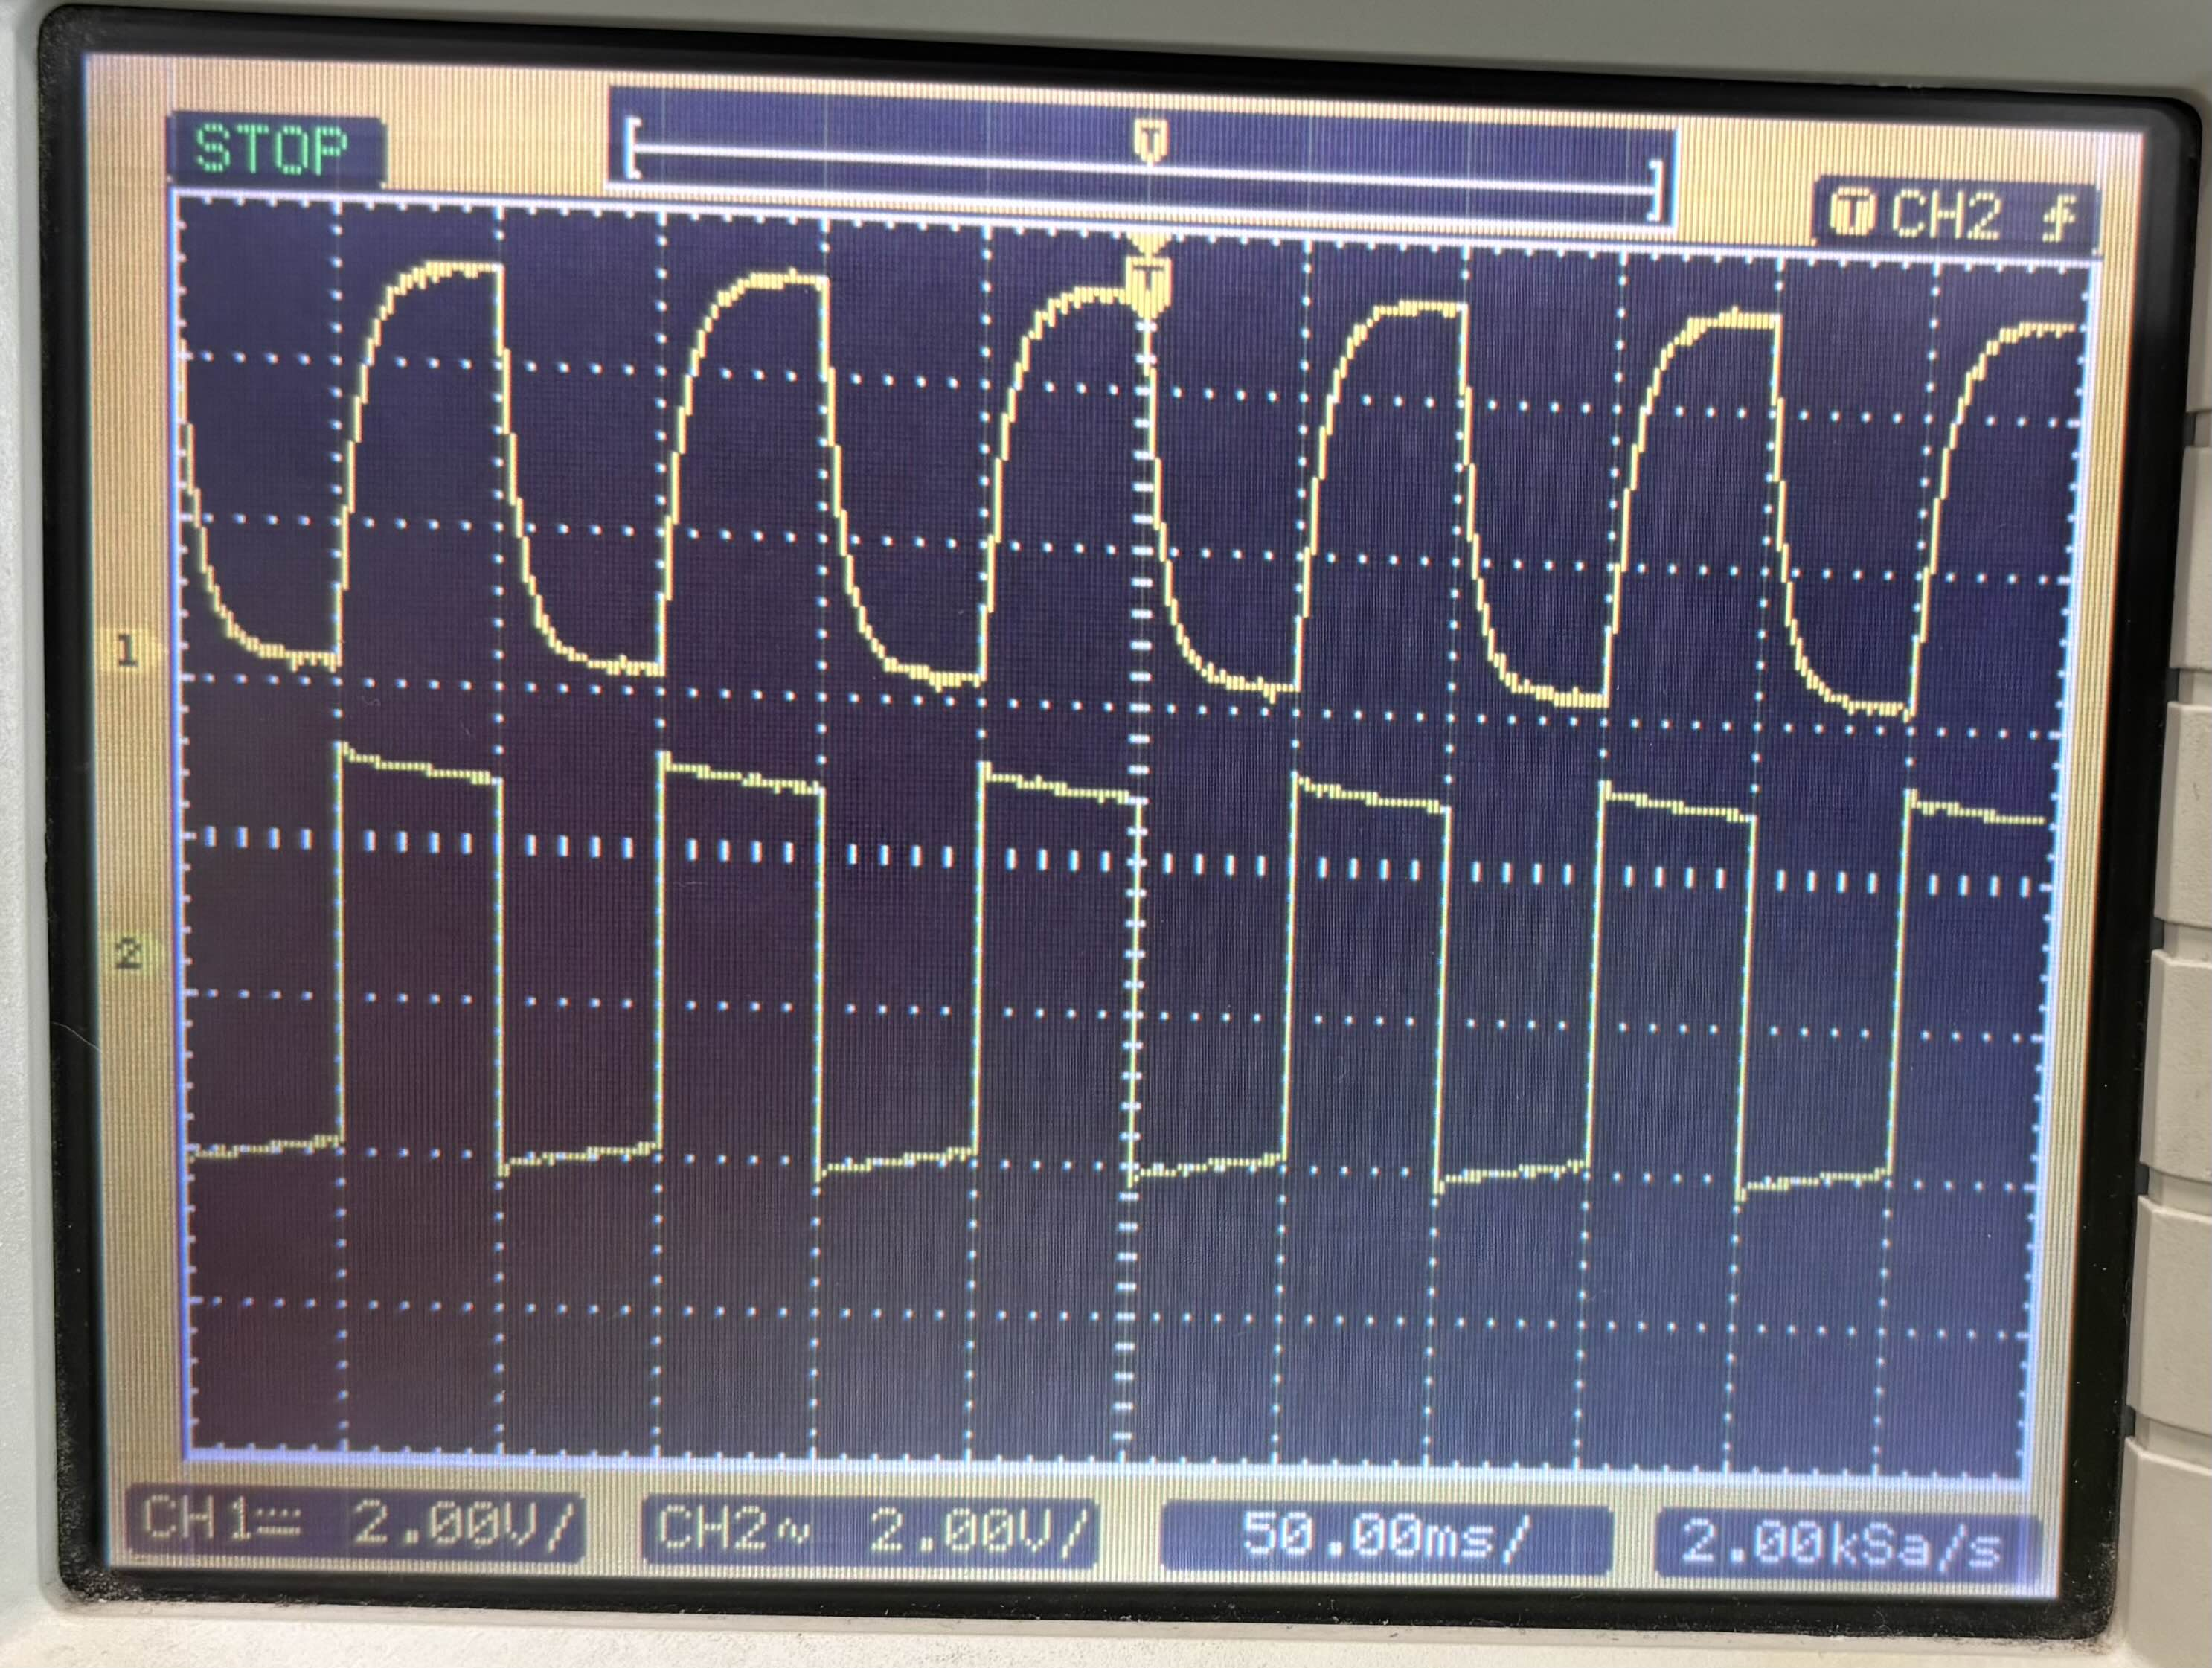
\includegraphics[ width=0.53\columnwidth]{figs/steady_1.jpg}}
    \hspace{\fill}
    {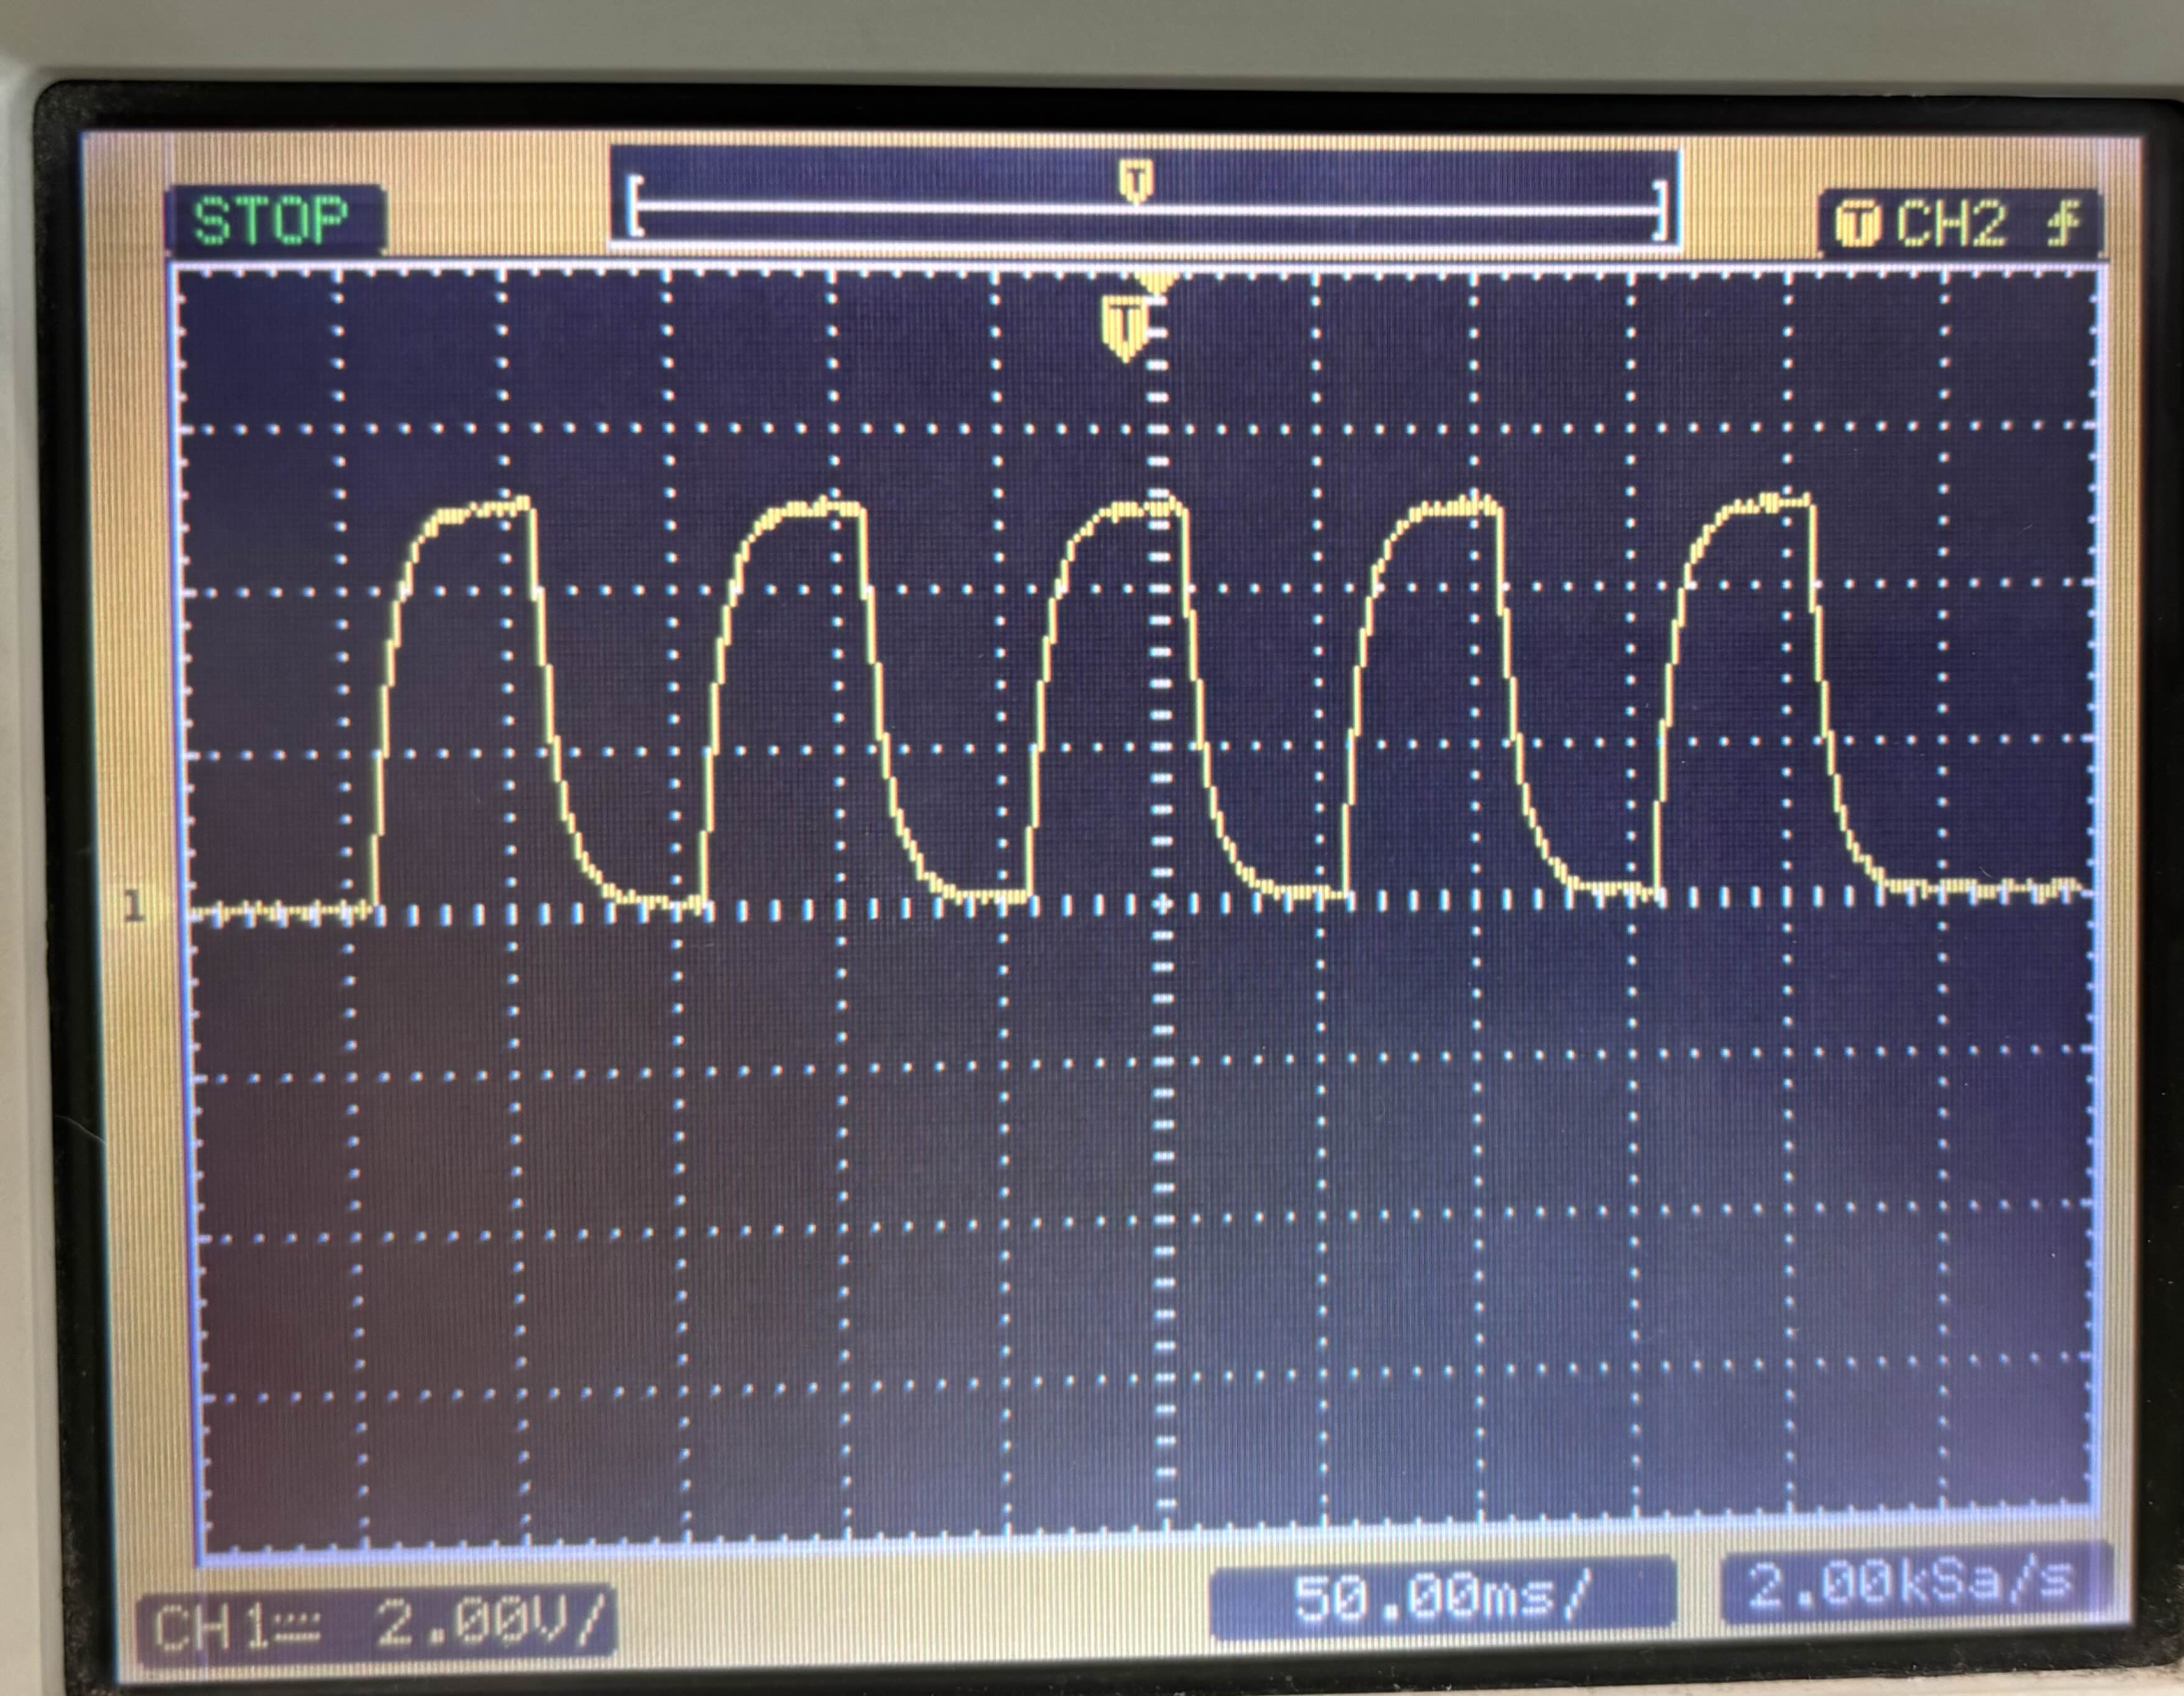
\includegraphics[ width=0.53\columnwidth]{./figs/trans_1.jpg}}
\end{figure*}

\subsection*{Case 2: \(RC = T\)}
\begin{figure*}[h!]
    {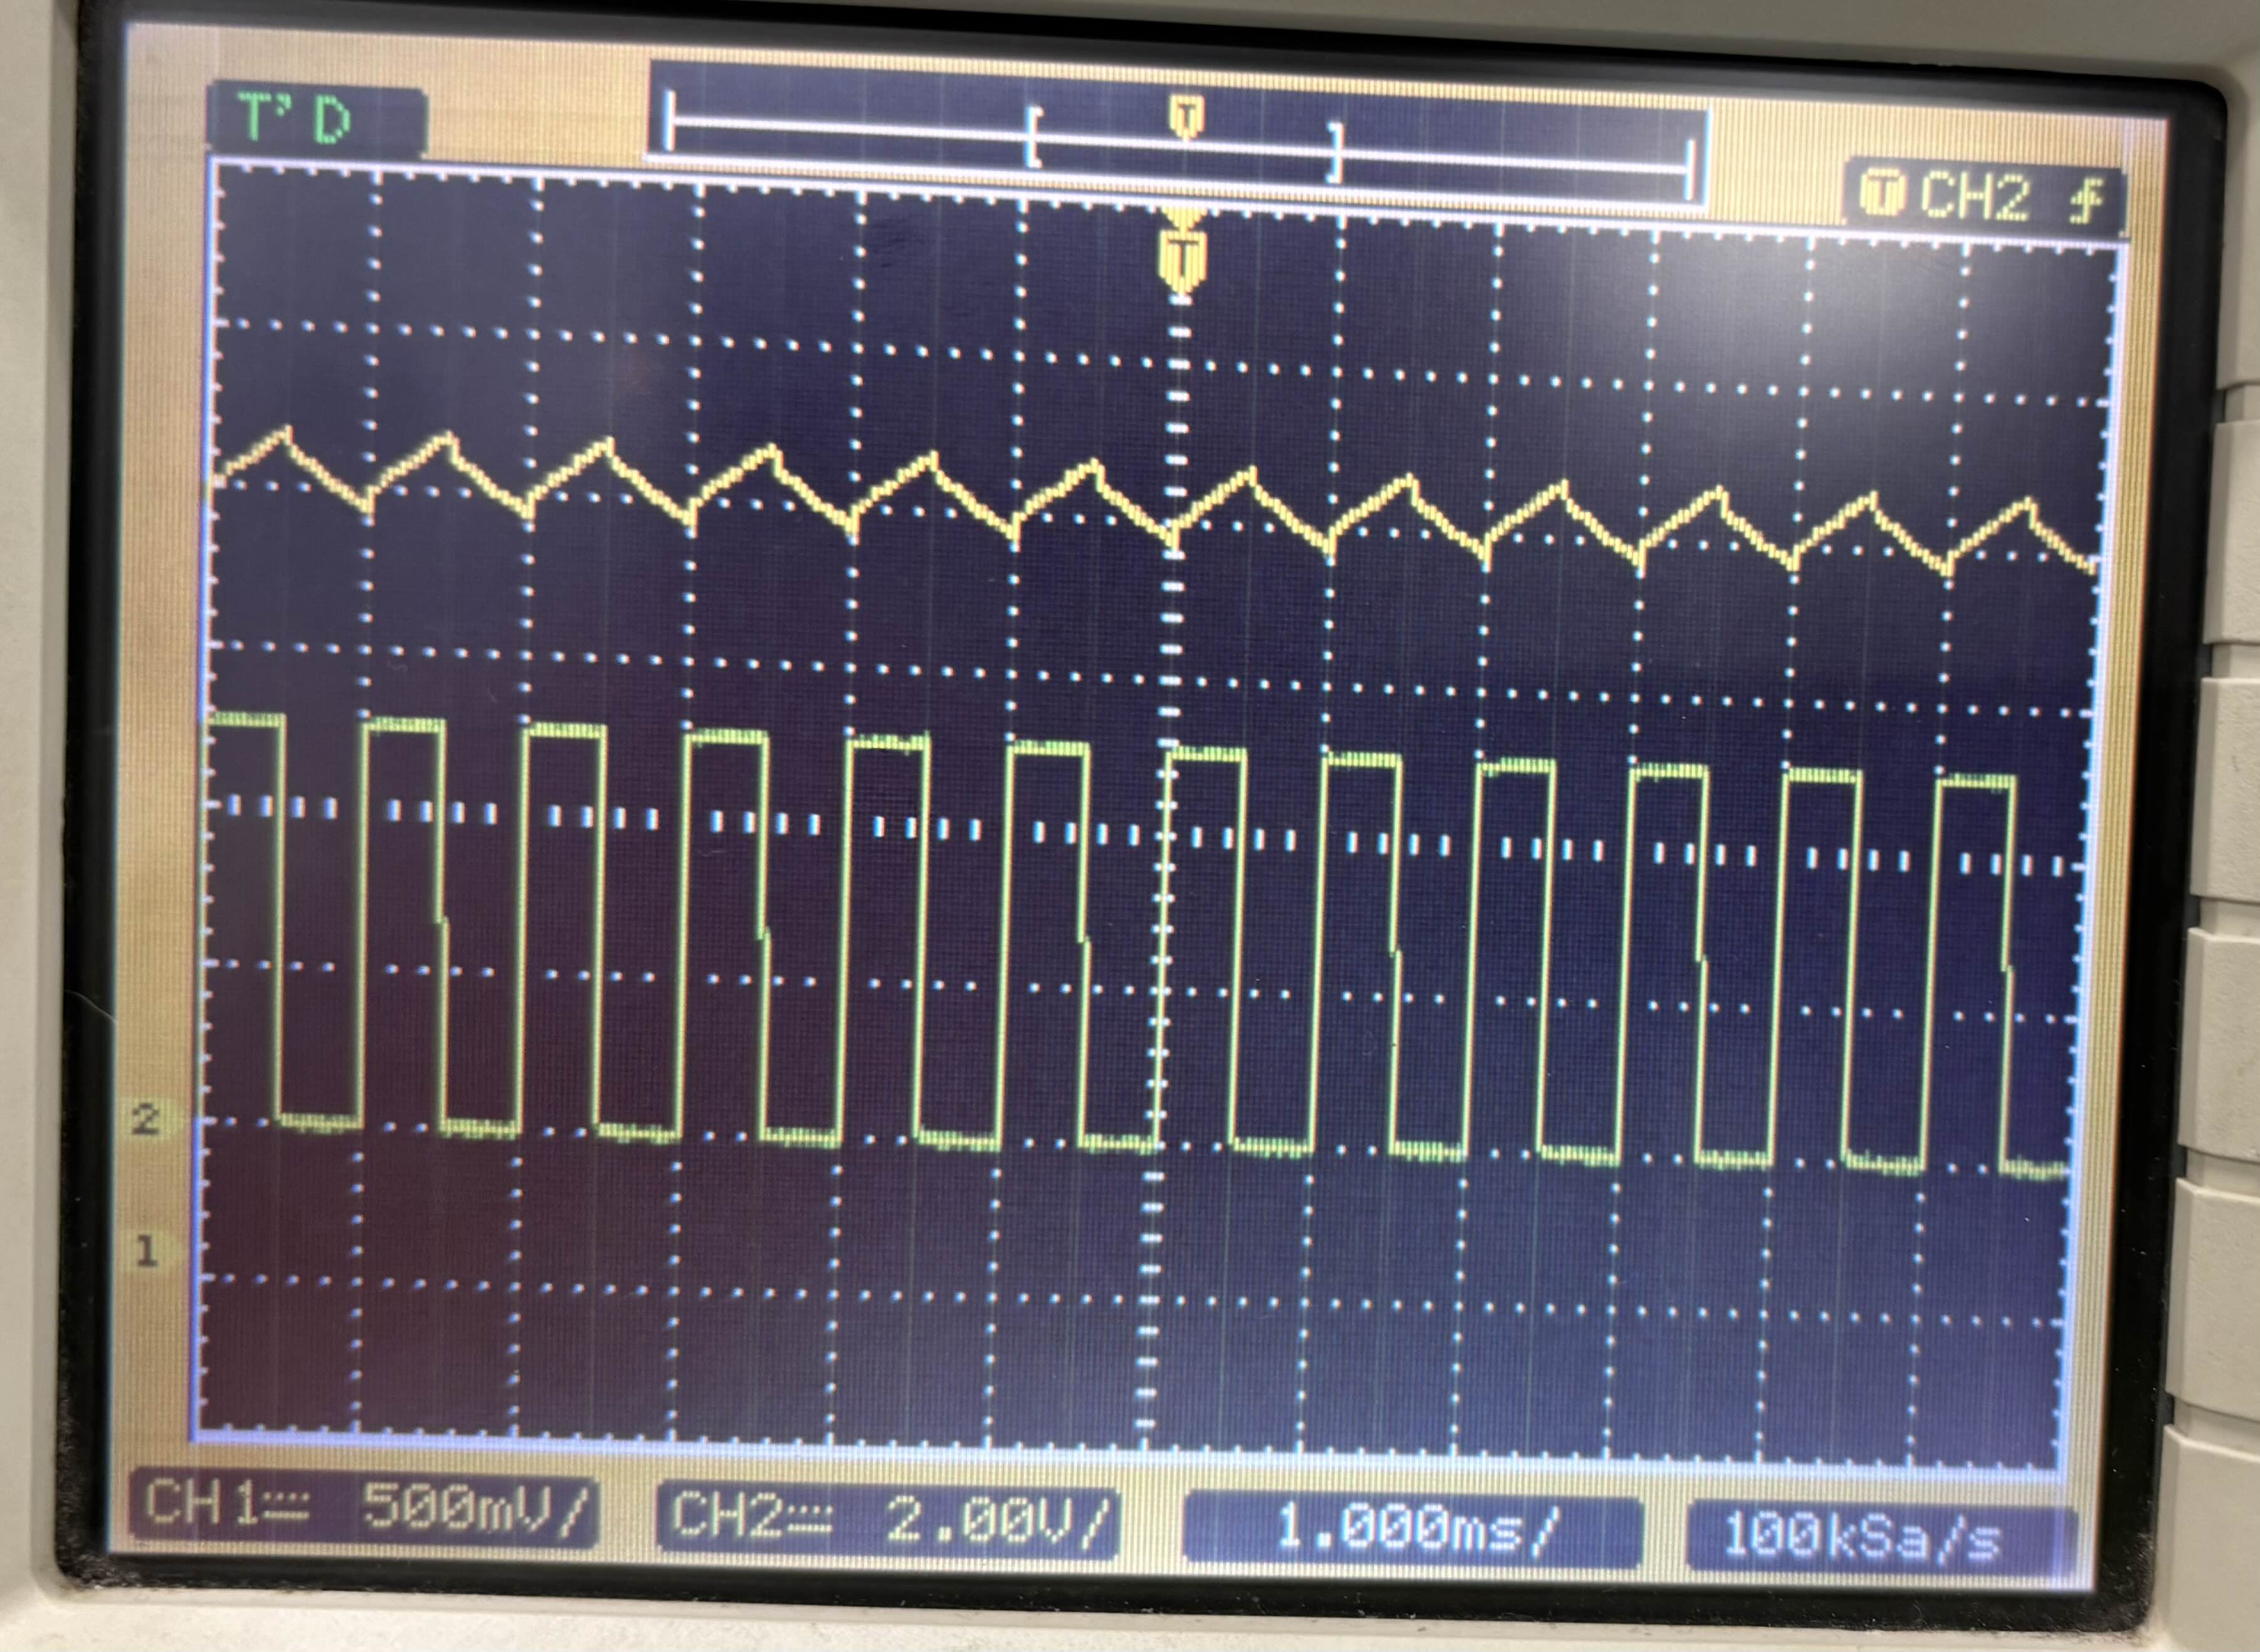
\includegraphics[ width=0.53\columnwidth]{figs/steady_2.jpg}}
    \hspace{\fill}
    {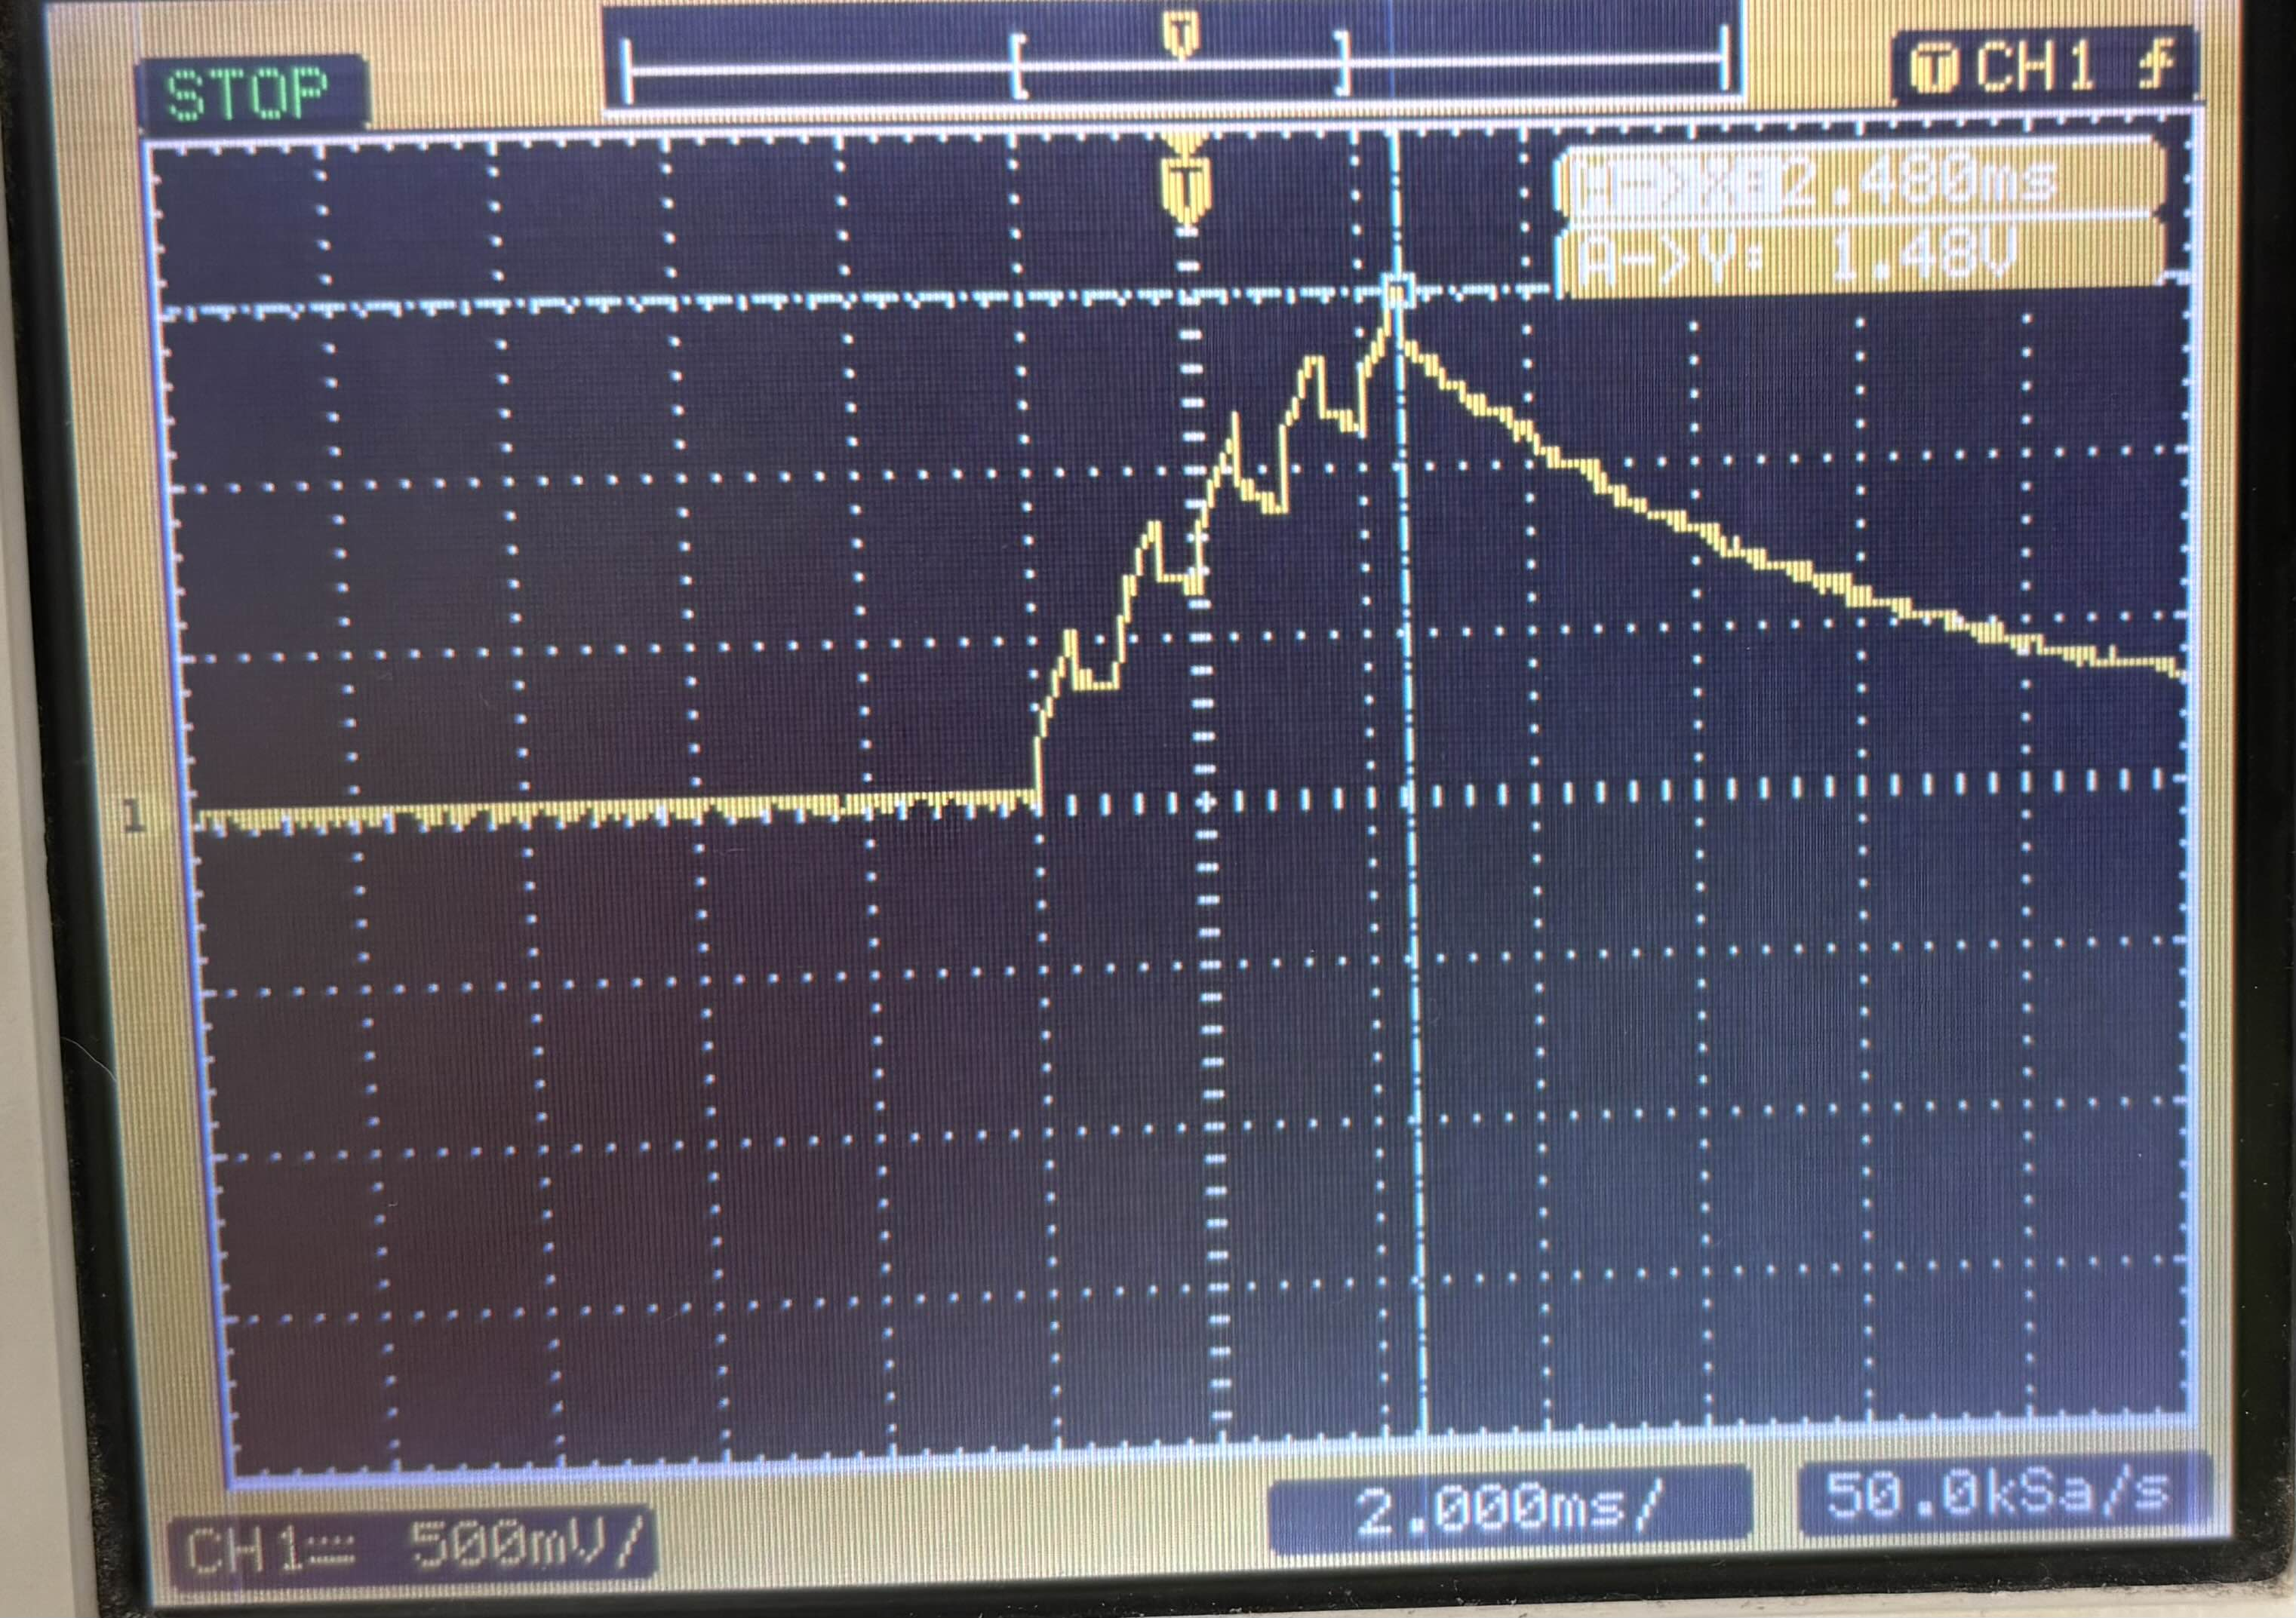
\includegraphics[ width=0.53\columnwidth]{./figs/trans_2.jpg}}
\end{figure*}

\subsection*{Case 3: \(RC >> T\)}
Here, we have plotted more than $5$ cycles of square wave as it better shows the increasing nature of the potential difference across capacitor. 
%\pagebreak
\begin{figure*}[h!]
    {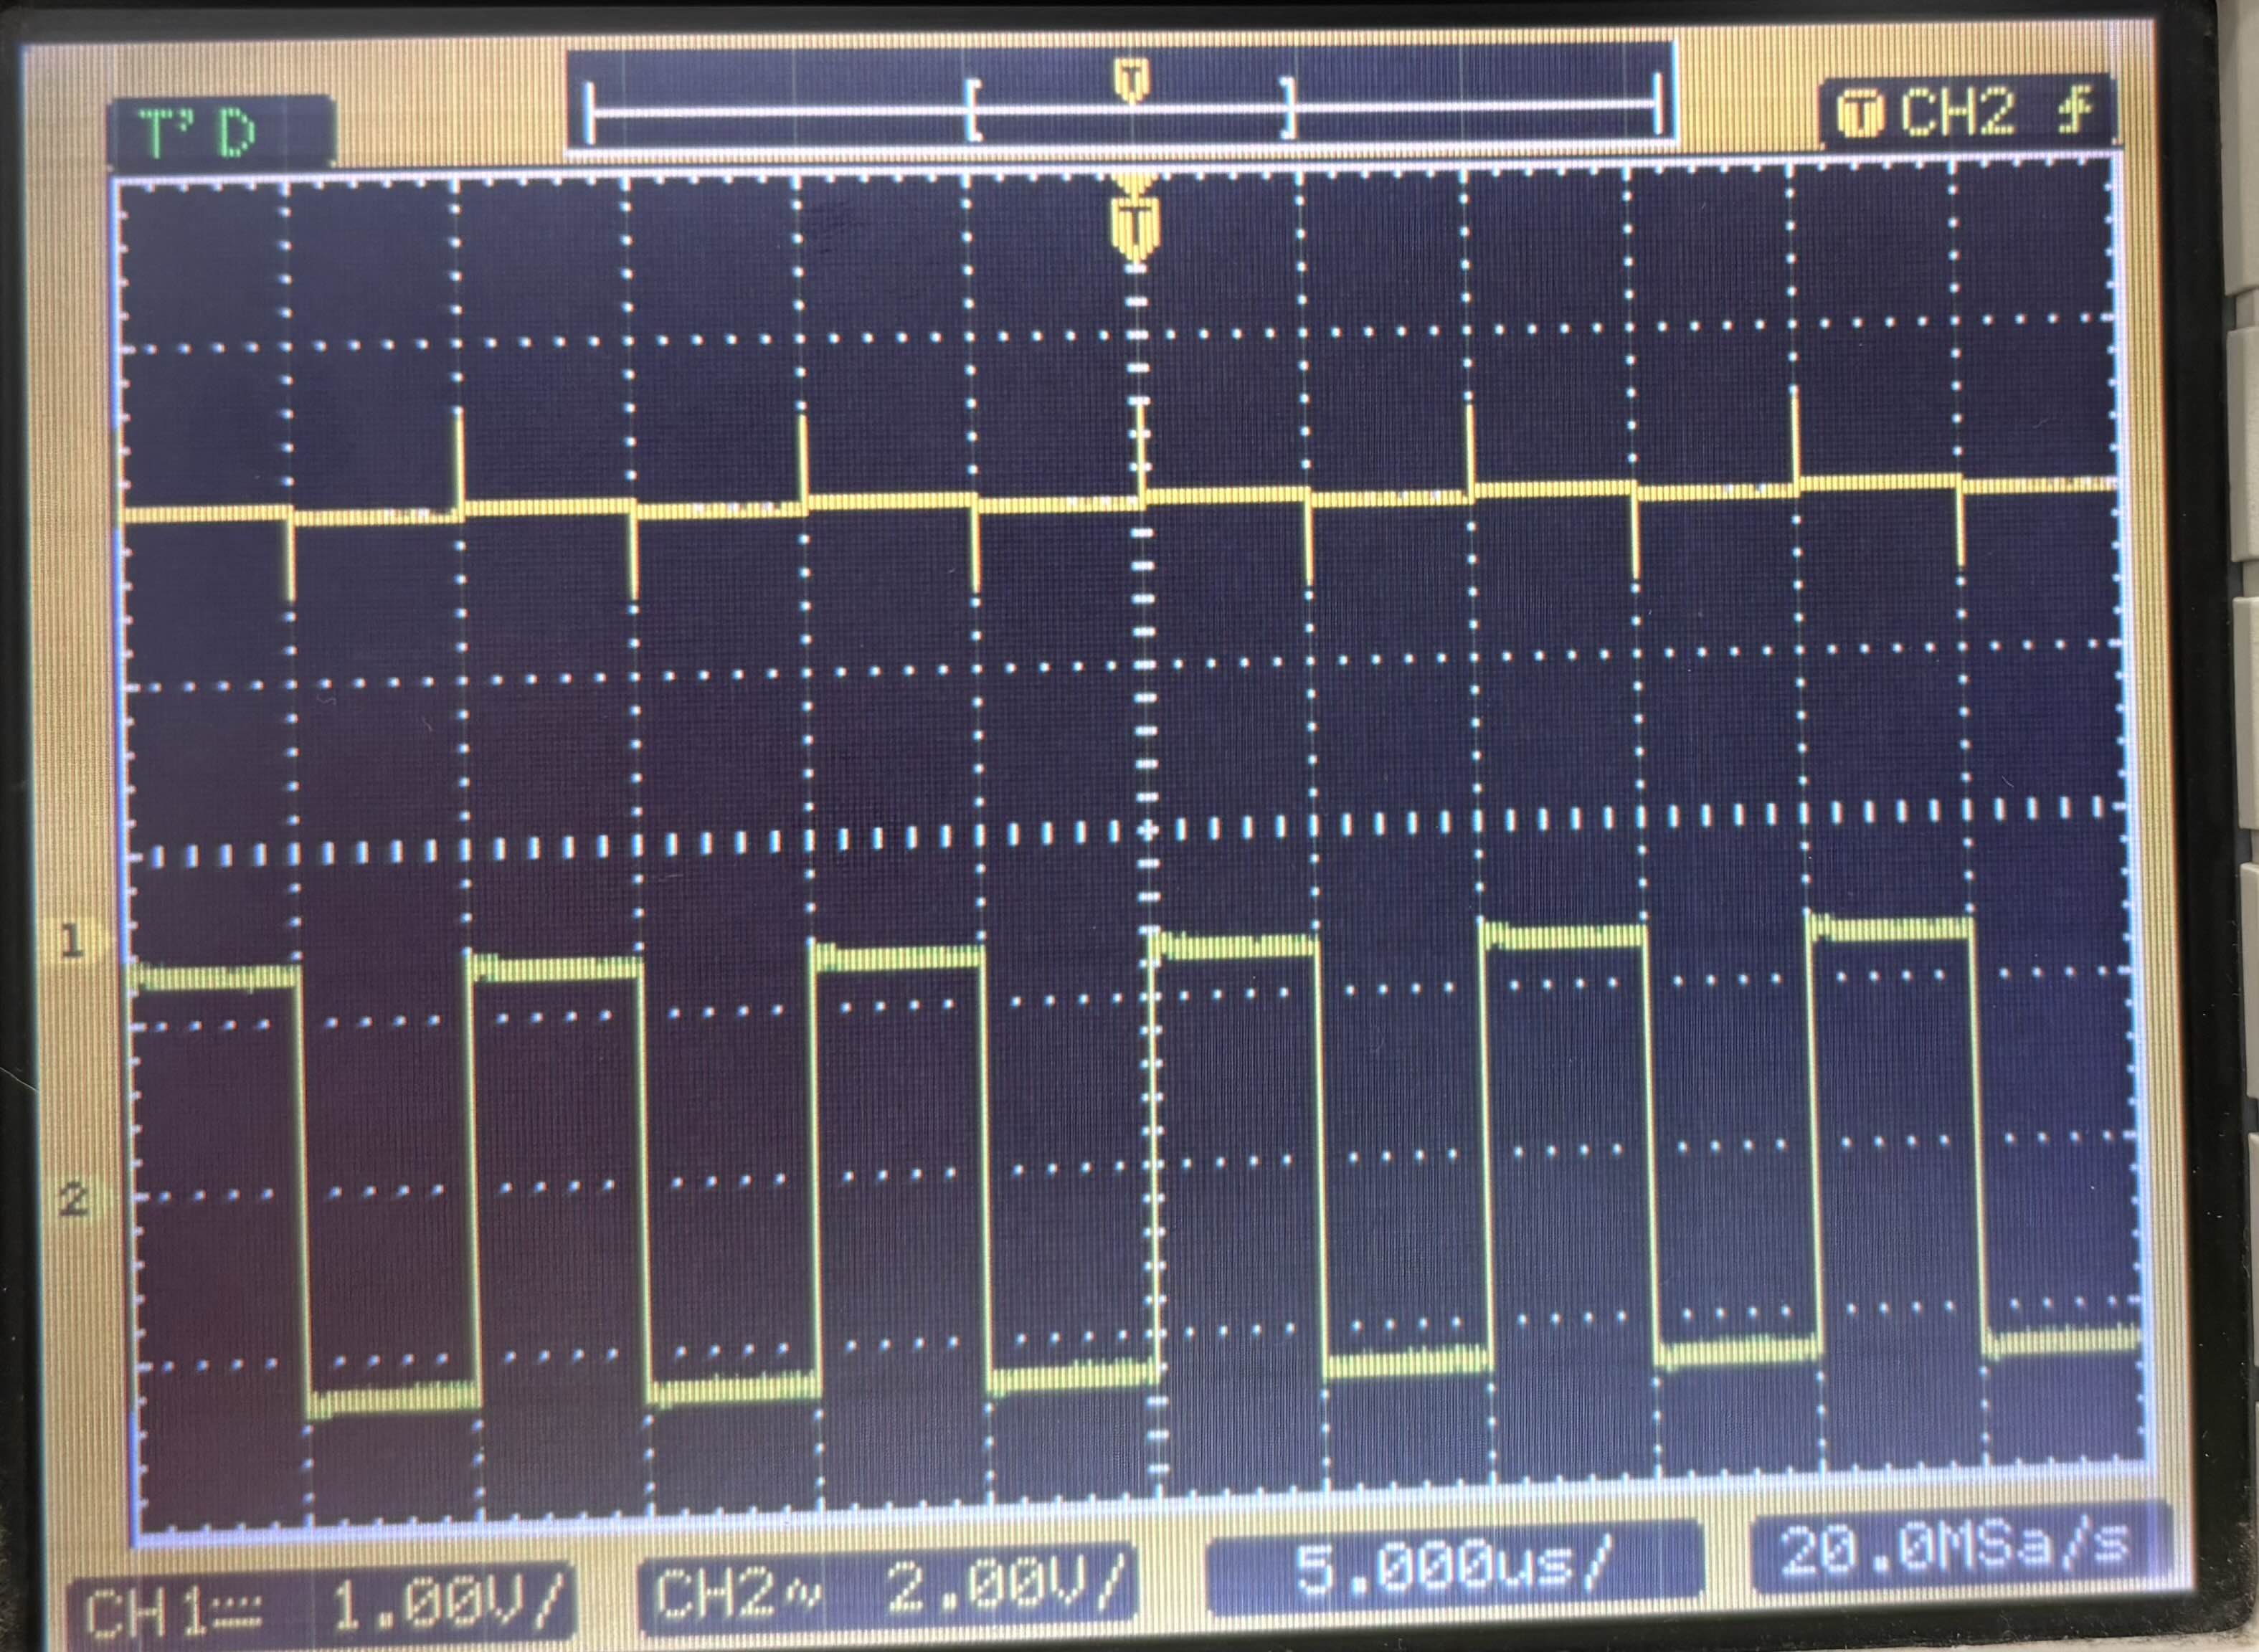
\includegraphics[ width=0.53\columnwidth]{figs/steady_3.jpg}}
    \hspace{\fill}
    {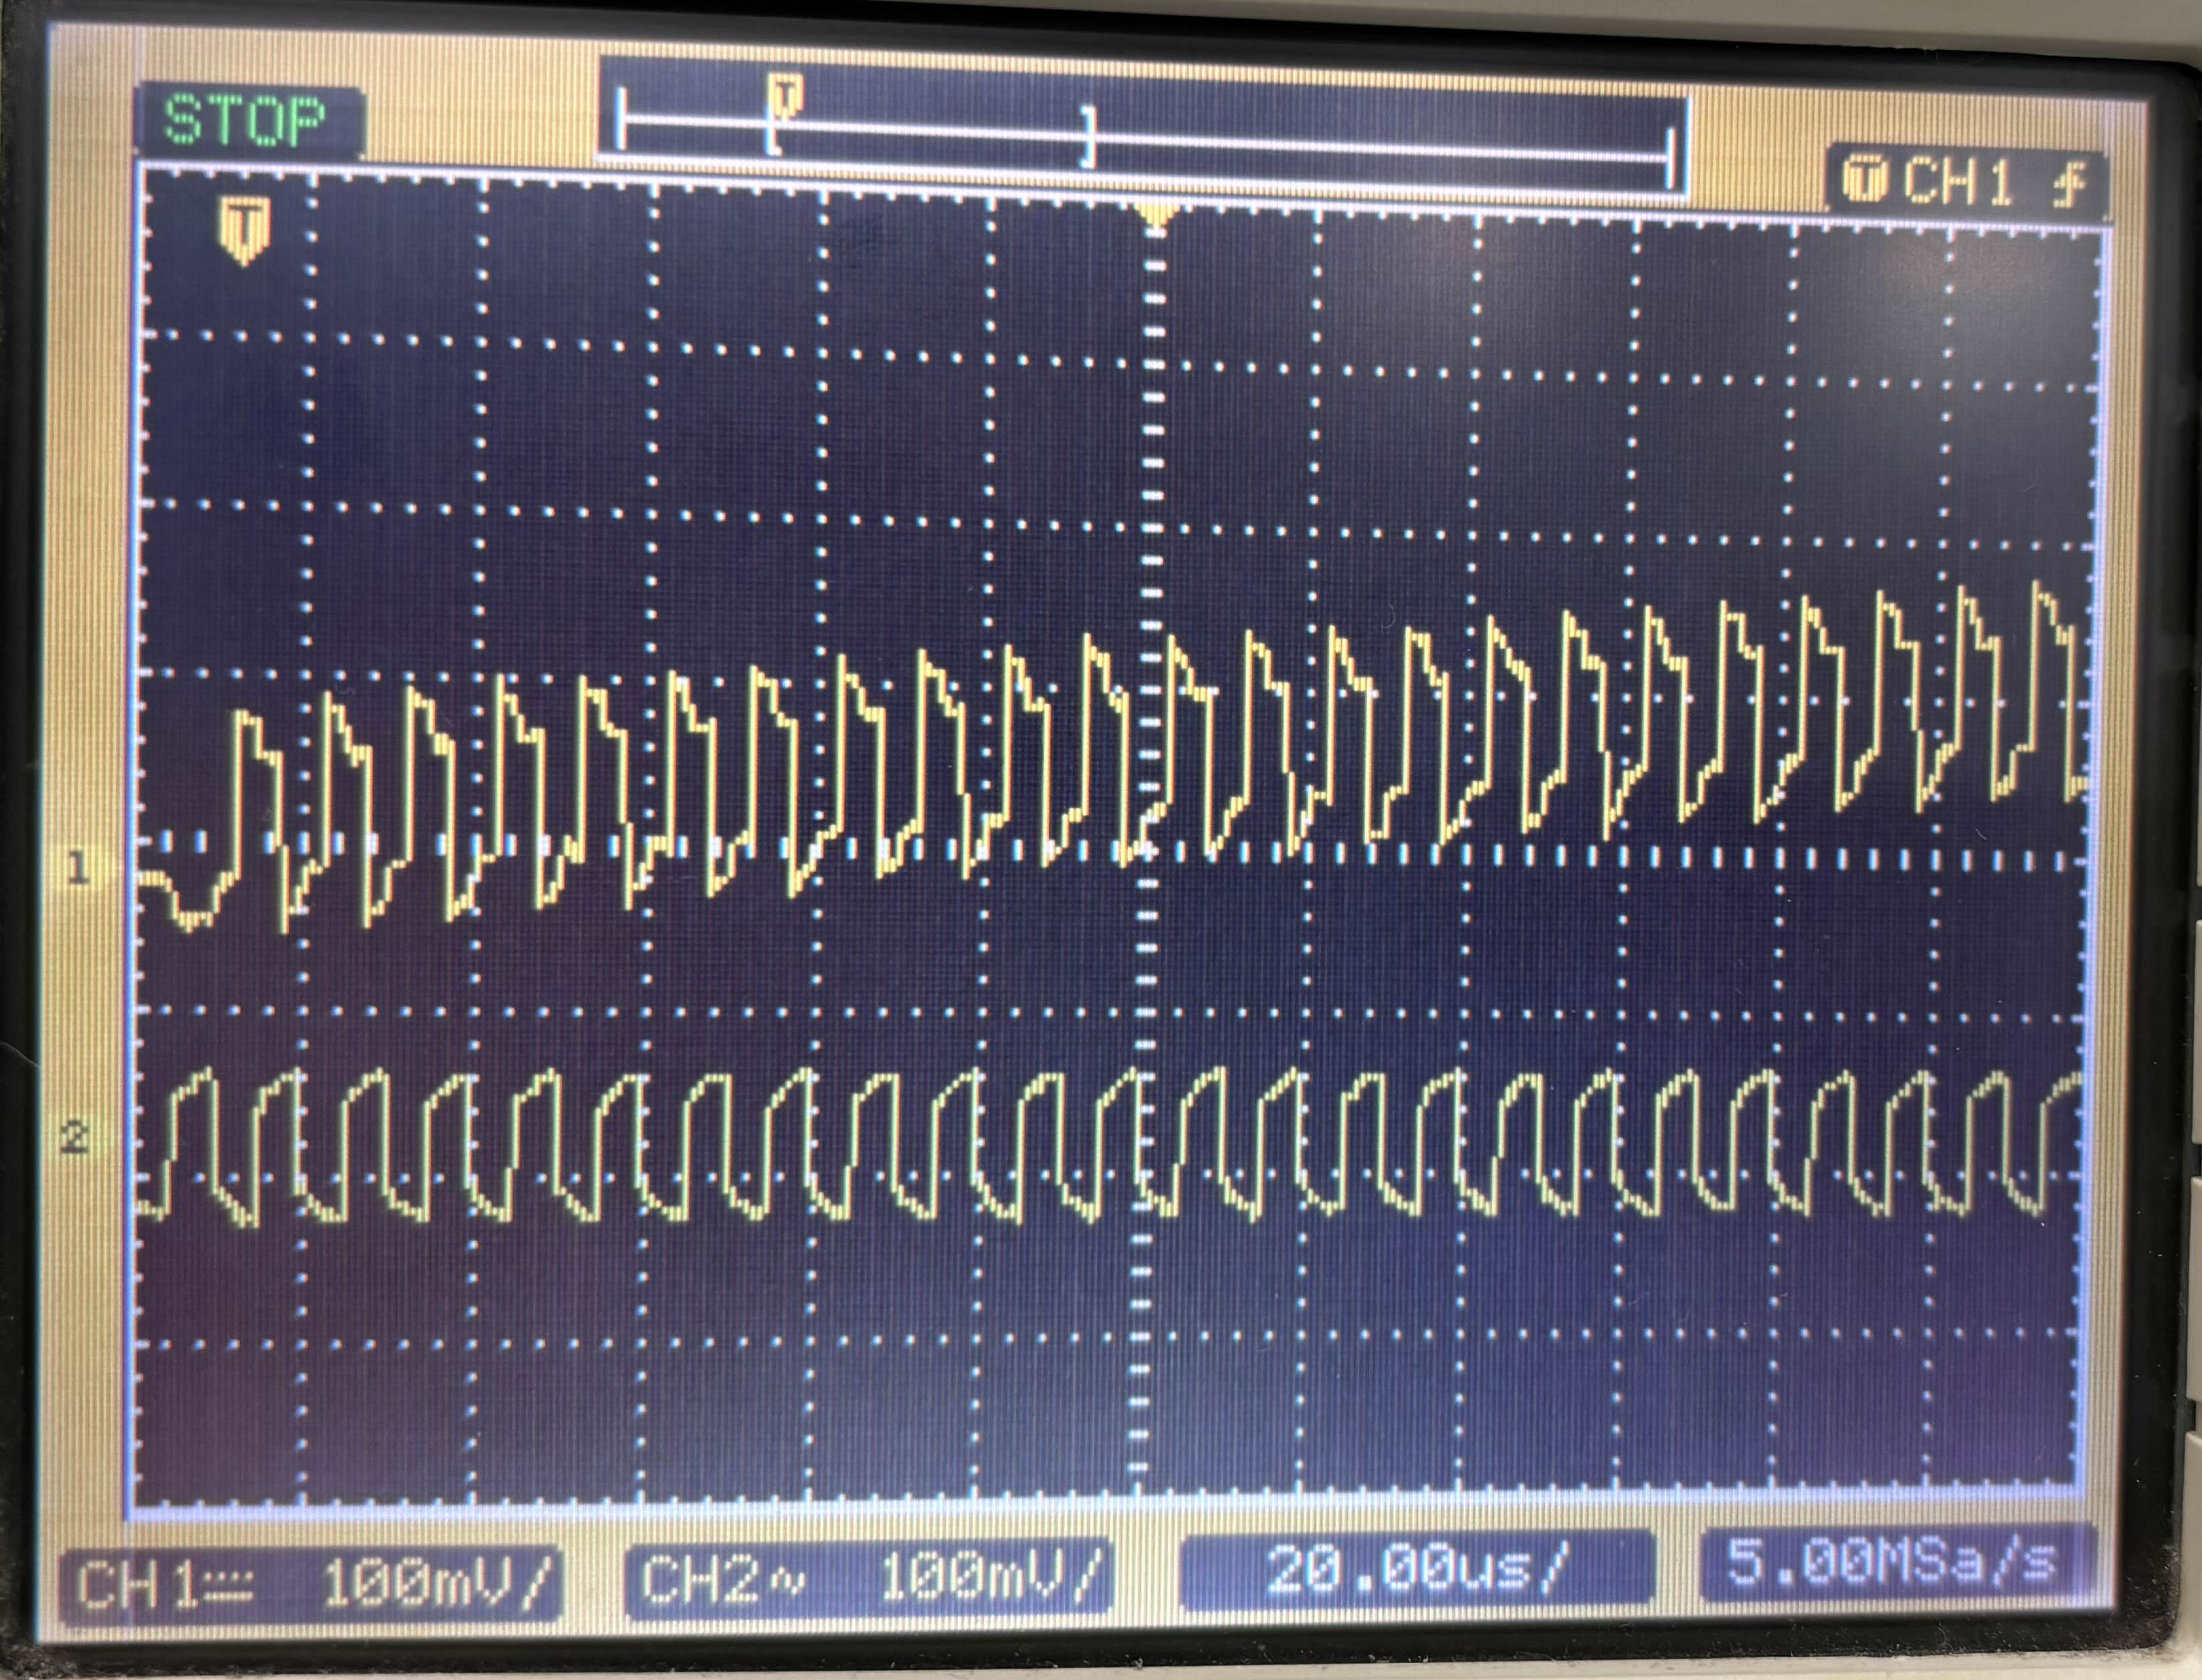
\includegraphics[ width=0.53\columnwidth]{./figs/trans_3.jpg}}
\end{figure*}\\
For an infinite number of cycles of square wave, output comes out to be,
\begin{figure}[h!]
  \centering
  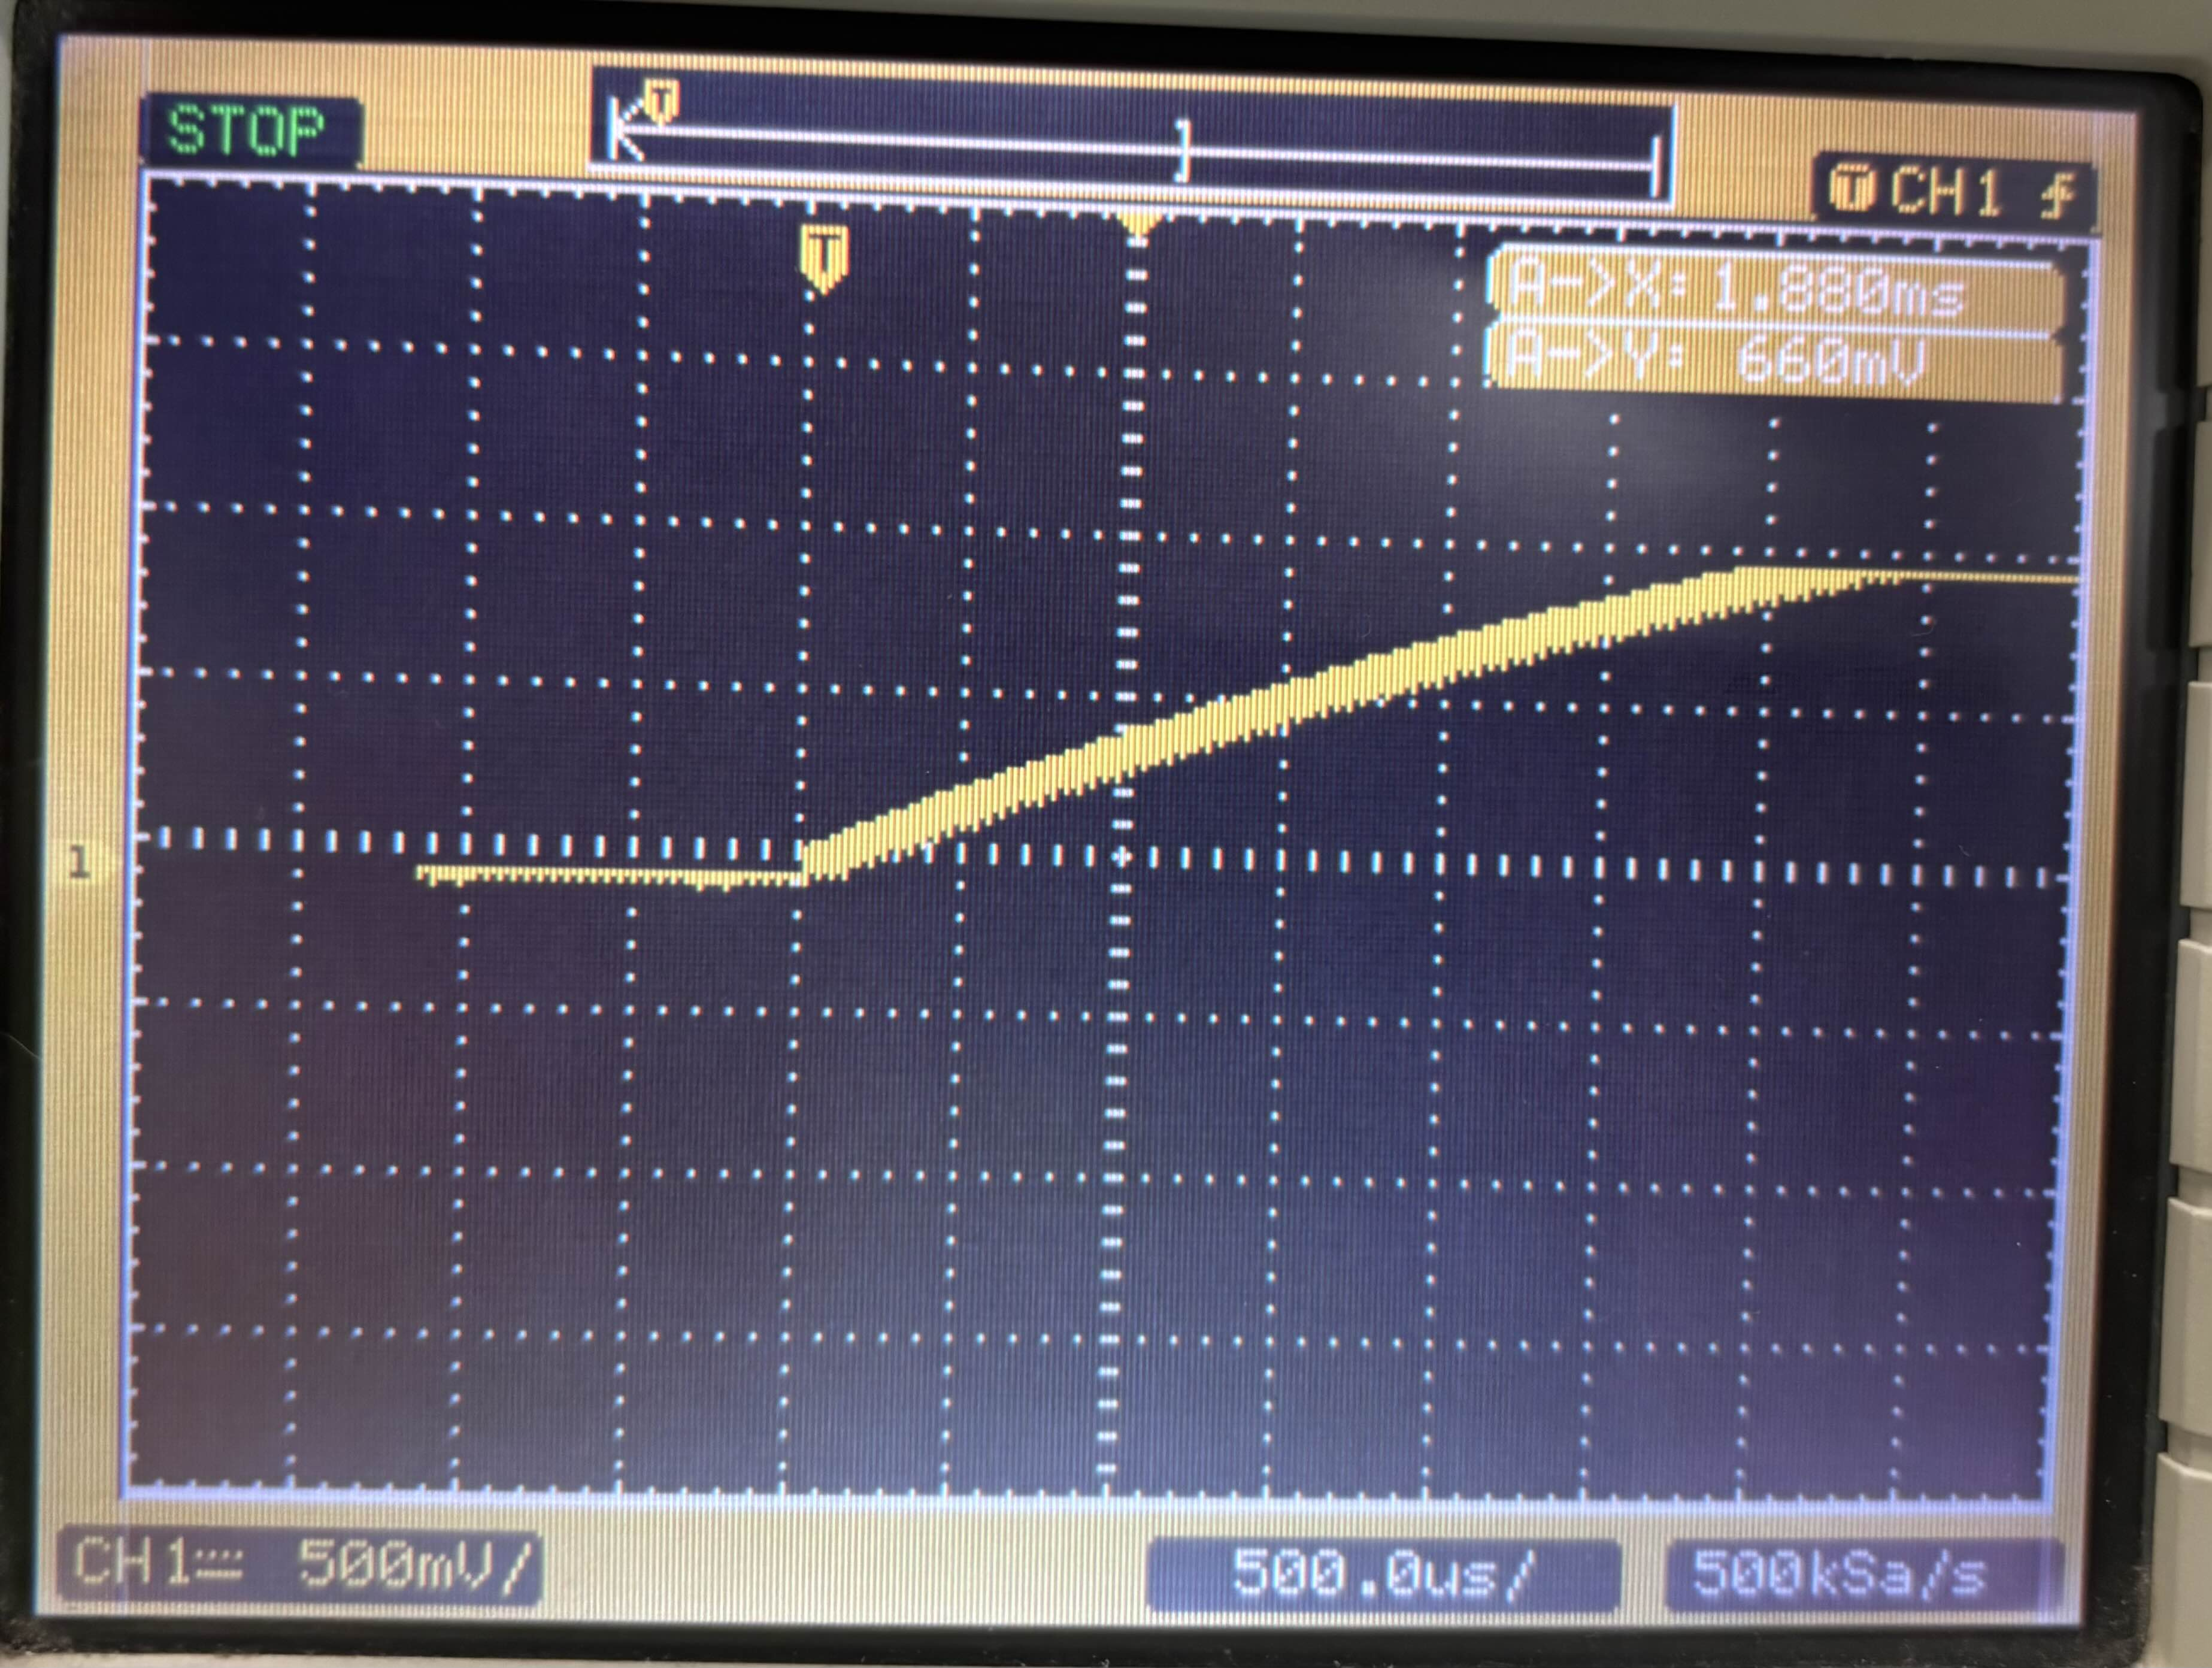
\includegraphics[width=0.7\columnwidth]{figs/trans_infty.jpg}
  \label{label}
\end{figure}
\section*{Discussion}
\begin{itemize}
    \item Compare the experimental results with the theoretical calculations.
    \item Discuss the effect of \(RC\) on the circuit response.
    \item Comment on any discrepancies between observed and theoretical values.
\end{itemize}

\section*{Conclusion}
The transient and steady-state behaviors of the RC circuit under a square wave input were successfully analyzed for the cases \(RC = T\), \(RC >> T\), and \(RC << T\). The observations matched the theoretical predictions within acceptable experimental error.
\end{document}


